% IEEE WCNC 2027 -- consumer-relative CSI certificate. IEEEtran conference class.
% Numbers are SEALED+GRADED (XPROTO-URLLC 2026-08-24; XPROTO-CSI + OT-14 2026-08-23),
% real 5G NR link-level (Sionna LDPC). Figures in ./build (300-dpi PNG from sealed data).
% Build: pdflatex wcnc-csi && bibtex? (embedded thebibliography) && pdflatex x2 (MiKTeX).
\documentclass[conference]{IEEEtran}
\usepackage{cite}
\usepackage{amsmath,amssymb}
\usepackage{graphicx}
\graphicspath{{./build/}}
\usepackage{textcomp}
\usepackage[colorlinks=true,allcolors=blue]{hyperref}

\begin{document}

\title{One CSI Report Cannot Serve Every Consumer:\\
The Consumer-Relative False-Clear Rate in 5G/6G Link Adaptation}

\author{\IEEEauthorblockN{Andrew H. Bond}
\IEEEauthorblockA{Department of Computer Engineering\\
San Jos\'e State University, San Jos\'e, CA, USA\\
andrew.bond@sjsu.edu}}

\maketitle

\begin{abstract}
A channel-state-information (CSI) report is a certificate: an implicit claim that the
channel is good enough to transmit at a selected rate. That certificate is not read by
the channel; it is read by a \emph{consumer}---a scheduler with a reliability target and
a decoder at a moment in time. We make the rate at which a CSI certificate
\emph{false-clears} (selects a rate the link cannot support) a first-class, measured KPI
on a real 5G~NR link-level chain (Sionna LDPC decoding), and show it is
\emph{consumer-relative} along two axes. First, the reliability target: the identical
CSI-derived modulation-and-coding selection that meets an eMBB target
($\mathrm{BLER}=10^{-1}$) misses a URLLC target ($10^{-3}$) by more than two orders of
magnitude ($112\times$), while a target-aware policy meets it. Second, the refresh
horizon: as the report ages, the false-clear rate grows, and the largest safe report
period is proportional to the Clarke coherence time ($\approx 0.177\,T_{\mathrm{coh}}$,
$R^2=0.915$). The witnessed corrections that hold each axis---outer-loop link adaptation,
a coherence-driven refresh---already exist; our contribution is the measured number that
says when each is needed. All results are drawn from sealed, pre-registered records.
\end{abstract}

\begin{IEEEkeywords}
CSI feedback, link adaptation, URLLC, outer-loop link adaptation, reliability, 5G NR.
\end{IEEEkeywords}

\section{Introduction}
Adaptive modulation and coding (AMC) turns a channel-state-information (CSI) report into
a rate decision: the transmitter selects the highest modulation-and-coding scheme (MCS)
whose required SINR the reported CSI clears. The report is thus a \emph{certificate}---an
implicit assertion that the link will decode at the chosen rate. Like any certificate,
it can be wrong in a way that matters only to whoever reads it. We call a wrong-in-the-
optimistic-direction certificate a \emph{false-clear}: the CSI cleared an MCS that the
true channel cannot support, and the transport fails (a HARQ NACK, a block error).

Our thesis is that the false-clear rate is not a property of the channel or even of the
report alone; it is a property of the report \emph{and its consumer}. Two schedulers
reading the same CSI can disagree on whether it false-clears, because they read it
against different requirements. We make the false-clear rate a measured KPI on a real
5G~NR link-level chain and demonstrate this consumer-relativity along two operationally
important axes:
\begin{itemize}
\item \textbf{the reliability target} (\S\ref{sec:urllc}): a single CSI-derived MCS that
is adequate for enhanced mobile broadband (eMBB) is catastrophically optimistic for
ultra-reliable low-latency communication (URLLC), by more than $100\times$;
\item \textbf{the refresh horizon} (\S\ref{sec:refresh}): the false-clear rate grows as
the certificate ages, and the safe refresh period scales with the channel coherence
time by a simple measured law.
\end{itemize}
Neither observation requires a new estimator or scheduler. The corrections are known:
outer-loop link adaptation (OLLA)~\cite{olla} closes the target-relativity gap, and
coherence-driven CSI reporting closes the refresh gap. What has been missing is the
\emph{measured, consumer-relative false-clear rate} that quantifies when each correction
is load-bearing and how large the exposure is when it is absent.

\section{Method}
\textbf{Substrate.} We use a real 5G~NR link-level chain in
Sionna~\cite{sionna}: LDPC-coded QAM over the NR PDSCH, with block error rate (BLER)
measured from the actual LDPC decoder rather than an SINR-to-BLER formula. The decoder
is the \emph{witness}: it independently determines whether the consumer decoded.

\textbf{Certificate, consumer, witness.} An AMC certificate selects the highest MCS whose
required SINR the CSI clears at a given BLER target. The \emph{consumer} is that rate
decision under a specific reliability target; the \emph{witness} is the LDPC decode
outcome. A false-clear is a certificate that clears an MCS the witness then fails.

\textbf{Discipline.} Each experiment is pre-registered with numerical bars and
manipulation checks fixed before the graded run; the sealed record is content-hashed and
graded on seeds disjoint from those used to design it, and negative or failing outcomes
are kept~\cite{otcampaigns}. The numbers below are the graded, sealed values.

\section{Consumer-Relativity in the Reliability Target}
\label{sec:urllc}
A base station serving mixed traffic derives one CSI estimate per user and selects an
MCS. Consider the same estimate consumed under two targets: eMBB
($\mathrm{BLER}\le 10^{-1}$) and URLLC ($\le 10^{-3}$). We drive a real NR link at high
mobility, apply the naive CSI-derived MCS, and measure the achieved BLER against each
target; we then compare a \emph{target-aware} policy that sizes its margin to the
consumer's target.

Figure~\ref{fig:urllc} reports the sealed result (three graded seeds). The naive
certificate achieves $\mathrm{BLER}\approx 0.112$. Read by the eMBB consumer this is at
target---the certificate is sound. Read by the URLLC consumer the \emph{same} $0.112$ is
a false-clear by $112\times$ (against $10^{-3}$): every such block is a reliability-SLA
violation, invisible to a scheduler that assumed one CSI report serves all traffic. The
target-aware policy---the same CSI, an added $\approx 2$\,dB margin sized to the URLLC
target---achieves $\mathrm{BLER}\approx 1.2\times10^{-5}$, comfortably within target, at
the cost of that margin's spectral efficiency. No single margin is correct for both
consumers: the eMBB-adequate margin fails URLLC, and the URLLC-safe margin over-provisions
eMBB. The false-clear rate is the number that prices the difference.

\begin{figure}[t]
  \centering
  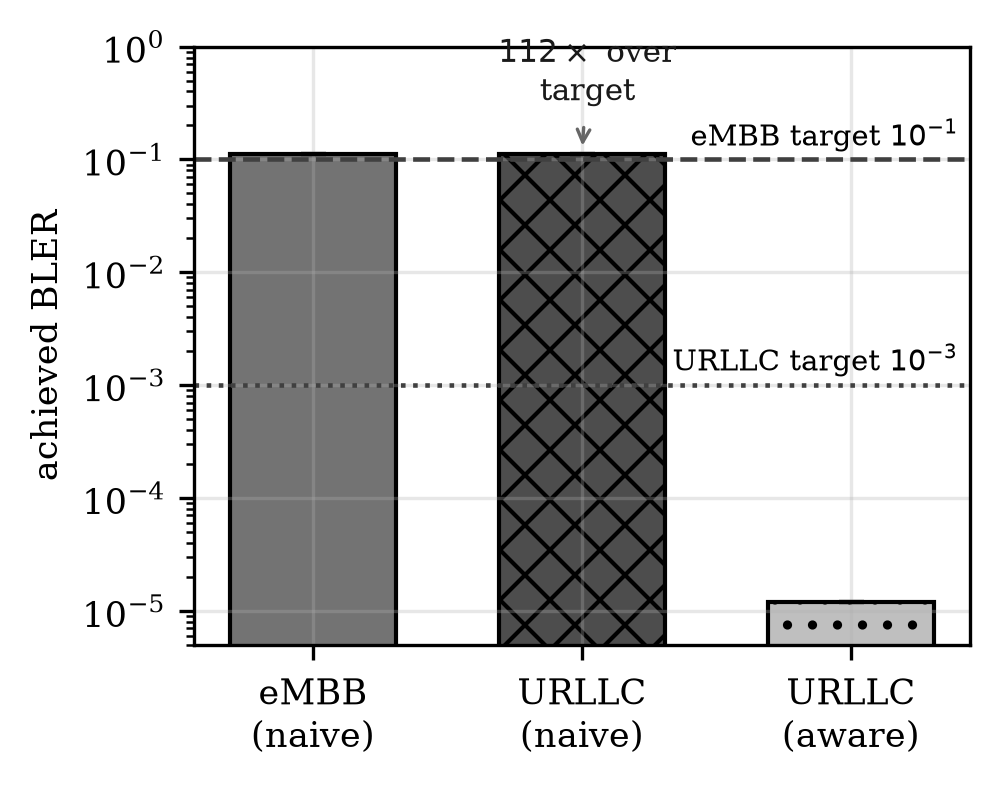
\includegraphics[width=0.82\linewidth]{urllc_relativity.png}
  \caption{Consumer-relativity of the CSI certificate in the reliability target
  (real NR, Sionna LDPC; three sealed seeds). The identical CSI-derived MCS meets the
  eMBB target ($10^{-1}$) but false-clears the URLLC target ($10^{-3}$) by $112\times$;
  a target-aware policy meets URLLC at the cost of $\sim$2\,dB margin.}
  \label{fig:urllc}
\end{figure}

\section{The Refresh Horizon}
\label{sec:refresh}
The second axis is time. A CSI report is fresh when issued and ages as the channel
decorrelates; a certificate that was sound at report time false-clears once the channel
has moved. At $f_D = 200$\,Hz with a $20$-TTI report period, the naive (held-CSI)
certificate reaches $\mathrm{BLER}\approx 0.36$ against a $0.1$ target---a false-clear on
roughly a quarter of transmissions---while OLLA, the deployed witnessed correction that
adjusts an offset from HARQ feedback, holds it at $\approx 0.10$
(Fig.~\ref{fig:refresh}(a) shows the aging across mobility).

The operational question is how often to refresh. Sweeping Doppler and report period,
we define the \emph{refresh floor} as the largest report period keeping BLER at target,
and find it proportional to the Clarke coherence time
$T_{\mathrm{coh}}=0.423/f_D$:
\begin{equation}
\text{refresh floor} \;\approx\; 0.177\,T_{\mathrm{coh}}, \qquad R^2 = 0.915,
\label{eq:ot14}
\end{equation}
across an order of magnitude of mobility (Fig.~\ref{fig:refresh}(b)). At high Doppler the
floor saturates at the minimum report period (one TTI): the certificate cannot be
refreshed faster than the frame allows, so above a mobility threshold no reporting
cadence suffices and a witnessed (HARQ-driven) correction becomes mandatory rather than
optional. Equation~\eqref{eq:ot14} gives a concrete provisioning rule: re-report before
the channel decorrelates past $\approx 0.18\,T_{\mathrm{coh}}$, not on a fixed calendar.

\begin{figure}[t]
  \centering
  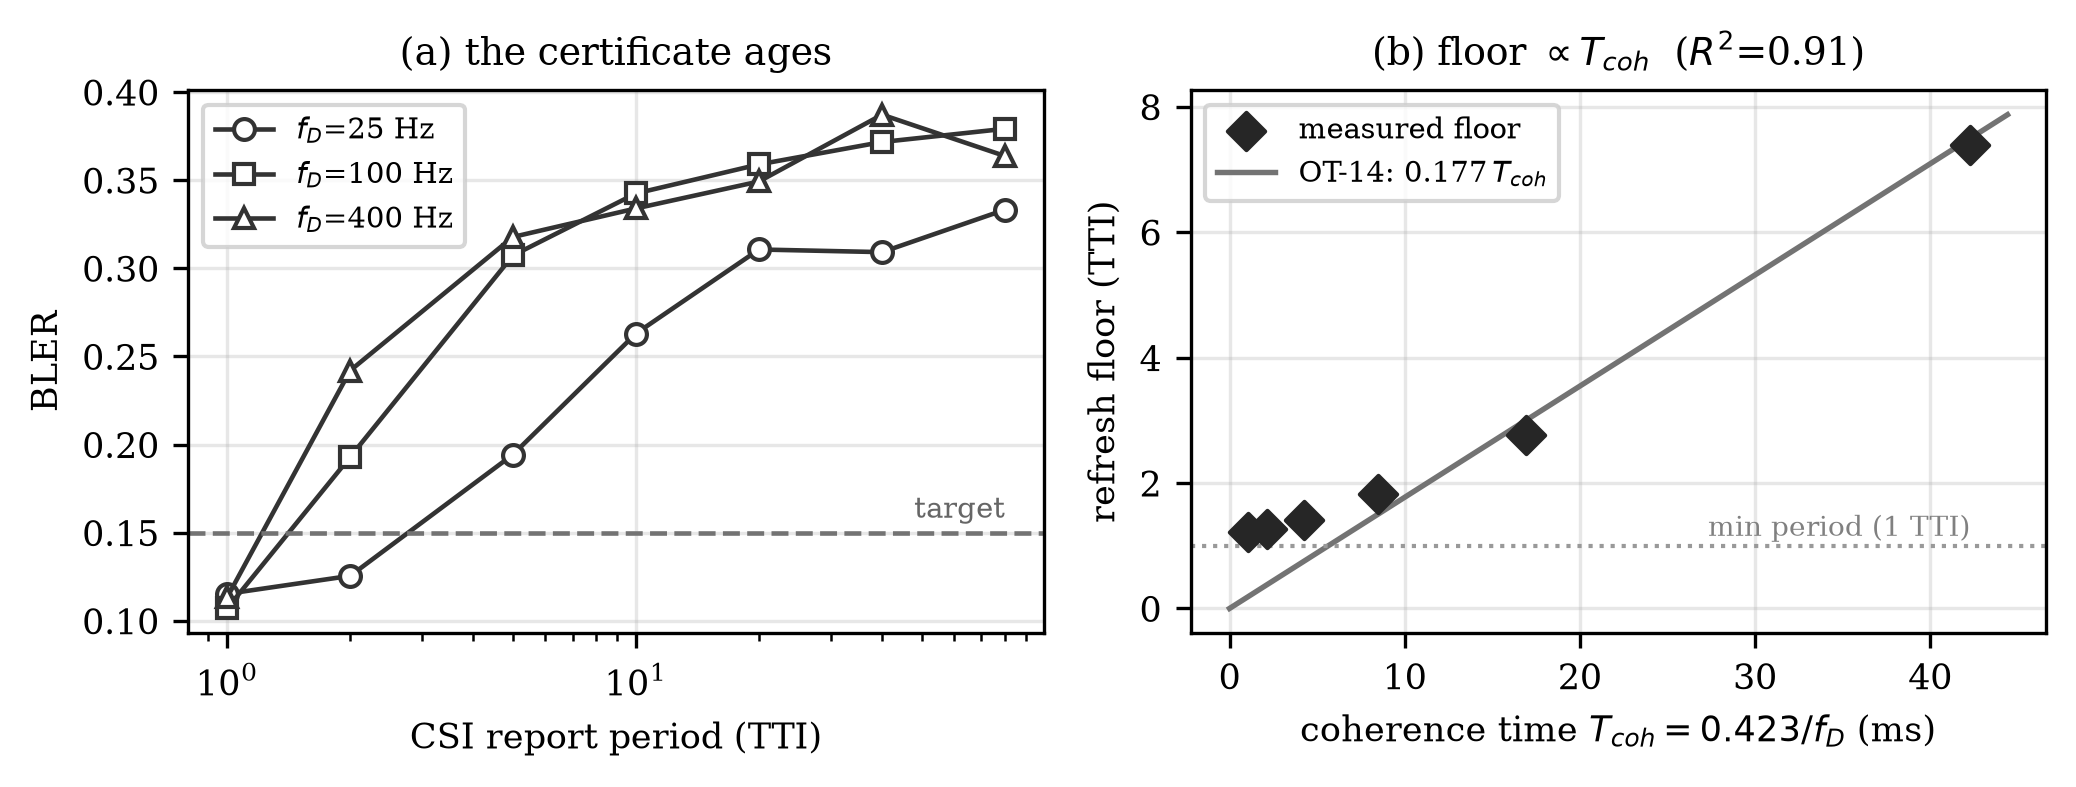
\includegraphics[width=\linewidth]{refresh_floor.png}
  \caption{The CSI certificate's refresh horizon (real NR, Sionna LDPC; sealed sweep).
  (a) The certificate ages: BLER grows with report period, faster at higher Doppler.
  (b) The refresh floor is proportional to the Clarke coherence time
  ($0.177\,T_{\mathrm{coh}}$, $R^2=0.915$); at high Doppler it saturates at one TTI.}
  \label{fig:refresh}
\end{figure}

\section{Related Work}
Link adaptation, CSI aging, and outer-loop correction are mature. OLLA~\cite{olla}
adjusts an SINR offset from HARQ ACK/NACK to hold a BLER target under imperfect or stale
CSI; it is precisely the witnessed correction our refresh-horizon result quantifies.
Short-packet and URLLC analysis~\cite{urllc} establishes the reliability-target regime in
which the eMBB-to-URLLC gap of \S\ref{sec:urllc} lives. Learned CSI feedback trained on
reconstruction error~\cite{csinet} is an active direction; we note only that the
reconstruction-versus-consumer objective gap it might imply did not appear at practical
operating points in our controlled tests, and we make no claim on it here. Our
contribution is orthogonal to all three: not a better estimator, scheduler, or offset
rule, but a \emph{measurement}---the false-clear rate as a first-class, consumer-relative
KPI---and the two relativities and the refresh law it exposes.

\section{Discussion and Conclusion}
The unit of correctness in link adaptation is not the CSI report but the pair (report,
consumer). Sizing margin and refresh cadence for the consumer's reliability target and
coherence time, rather than for a nominal channel, is what keeps a certificate honest.
The false-clear rate makes the cost of ignoring the consumer measurable: $112\times$ for a
mismatched target, a coherence-scaled horizon for a stale report. The Sionna link-level
chain is the evidence rung; an over-the-air or srsRAN testbed with real HARQ traces is the
external-validity graduation. The methodology is not radio-specific---the same
consumer-relative false-clear appears in optical quality-of-transmission and database
replication~\cite{otcampaigns}---but the results here stand on the 5G~NR CSI certificate
alone.

\begin{thebibliography}{1}
\bibitem{olla} A.~Sampath, P.~S.~Kumar, and J.~M.~Holtzman, ``On setting reverse link
target SIR in a CDMA system,'' in \emph{Proc. IEEE VTC}, 1997, pp.~929--933.
\bibitem{sionna} J.~Hoydis \emph{et al.}, ``Sionna: An open-source library for
next-generation physical layer research,'' arXiv:2203.11854, 2022.
\bibitem{urllc} G.~Durisi, T.~Koch, and P.~Popovski, ``Toward massive, ultrareliable, and
low-latency wireless communication with short packets,'' \emph{Proc. IEEE}, vol.~104,
no.~9, pp.~1711--1726, 2016.
\bibitem{csinet} C.-K.~Wen, W.-T.~Shih, and S.~Jin, ``Deep learning for massive MIMO CSI
feedback,'' \emph{IEEE Wireless Commun. Lett.}, vol.~7, no.~5, pp.~748--751, 2018.
\bibitem{otcampaigns} A.~H.~Bond, ``Observation Theory: consumer-relative witnessed
certificates,'' sealed pre-registrations and code,
\url{https://github.com/ahb-sjsu/observation-theory-campaigns}, 2026.
\end{thebibliography}

\end{document}
